\def\doctitle{Demo: Speaker}
\def\docsubtitle{Build, measure, and prove a paper-cup transducer}
\def\docstrap{changing current becomes motion and sound}
\def\materialslist{%
  \item Paper cup, card coil former, low-tack tape, paper flag
  \item 30--32 AWG insulated copper wire; sandpaper
  \item Ceramic magnet or adult-secured neodymium magnet
  \item Battery-powered, current-limited audio amplifier; tone source
  \item 100 \(\Omega\), 1 W series resistor; digital multimeter
  \item Ruler and optional phone spectrum display (observer only)}
\def\prediction{%
  Sketch what you expect for steady DC and for a slow alternating signal.
  Which part should move? Will doubling frequency double loudness? What
  measurement would distinguish ``the coil is open'' from ``the cone is stuck''?}

\def\diagram{%
\section{Construction plate}
\begin{center}
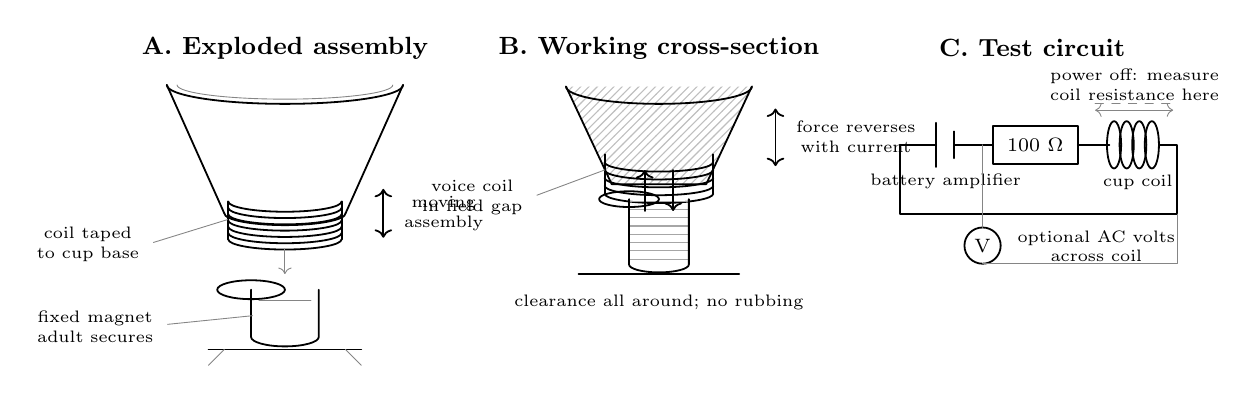
\begin{tikzpicture}[x=1cm,y=1cm,line cap=round,line join=round,
  ink/.style={draw=black,line width=.65pt},
  light/.style={draw=black!48,line width=.32pt},
  callout/.style={font=\fontsize{6.4}{7.1}\selectfont,align=center}]
% Exploded assembly.
\node[font=\small\bfseries] at (-4.75,2.05) {A. Exploded assembly};
\draw[ink](-6.25,1.58) arc (180:360:1.5 and .24);
\draw[ink](-6.25,1.58)--(-5.52,-.05);
\draw[ink](-3.25,1.58)--(-3.98,-.05);
\draw[light](-6.12,1.58) arc (180:360:1.37 and .18);
\draw[ink](-5.52,-.05) arc (180:360:.77 and .15);
\foreach \y in {-.38,-.30,...,.10}
  \draw[ink](-5.47,\y) arc (180:360:.72 and .13);
\draw[ink](-5.47,-.38)--(-5.47,.10) (-4.03,-.38)--(-4.03,.10);
\draw[->,light](-4.75,-.50)--(-4.75,-.82);
\draw[ink,fill=white](-5.18,-1.02) ellipse (.43 and .12);
\draw[ink](-5.18,-1.02)--(-5.18,-1.62)
  arc (180:360:.43 and .12)--(-4.32,-1.02);
\draw[light](-5.08,-1.16)--(-4.42,-1.16);
\draw[ink](-5.72,-1.78)--(-3.78,-1.78);
\draw[light](-5.52,-1.78)--(-5.72,-1.98)
  (-3.98,-1.78)--(-3.78,-1.98);
\draw[light](-5.48,-.13)--(-6.42,-.42);
\node[callout,anchor=e]at(-6.48,-.42){coil taped\\to cup base};
\draw[light](-5.16,-1.35)--(-6.24,-1.46);
\node[callout,anchor=e]at(-6.30,-1.46){fixed magnet\\adult secures};
\draw[<->,ink](-3.50,-.36)--(-3.50,.26);
\node[callout,anchor=west]at(-3.36,-.05){moving\\assembly};

% Section through magnetic gap.
\node[font=\small\bfseries] at (0,2.05) {B. Working cross-section};
\path[pattern=north east lines,pattern color=black!25]
  (-1.18,1.56)--(-.60,.32)--(.60,.32)--(1.18,1.56)--cycle;
\draw[ink](-1.18,1.56)--(-.60,.32)--(.60,.32)--(1.18,1.56);
\draw[ink](-1.18,1.56) arc (180:360:1.18 and .22);
\foreach \y in {.20,.30,...,.70}
  \draw[ink](-.69,\y) arc (180:360:.69 and .12);
\draw[ink](-.69,.20)--(-.69,.70) (.69,.20)--(.69,.70);
\path[pattern=horizontal lines,pattern color=black!35]
  (-.38,-.70) rectangle (.38,.13);
\draw[ink](-.38,.13) ellipse (.38 and .10);
\draw[ink](-.38,.13)--(-.38,-.70)
  arc (180:360:.38 and .10)--(.38,.13);
\draw[ink](-1.02,-.82)--(1.02,-.82);
\draw[->,ink](-.18,-.02)--(-.18,.50);
\draw[->,ink](.18,.50)--(.18,-.02);
\draw[<->,ink](1.48,.55)--(1.48,1.28);
\node[callout,anchor=west]at(1.62,.92){force reverses\\with current};
\draw[light](-.69,.50)--(-1.55,.18);
\node[callout,anchor=e]at(-1.61,.18){voice coil\\in field gap};
\node[callout]at(0,-1.18){clearance all around; no rubbing};

% Connection/checking circuit.
\node[font=\small\bfseries] at (4.74,2.05) {C. Test circuit};
\draw[ink](3.06,.82)--(3.52,.82);
\draw[ink](3.52,.54)--(3.52,1.10);
\draw[ink](3.75,.65)--(3.75,.99);
\node[callout]at(3.64,.36){battery amplifier};
\draw[ink](3.75,.82)--(4.24,.82);
\draw[ink](4.24,.58) rectangle (5.32,1.06);
\node[font=\scriptsize]at(4.78,.82){100 \(\Omega\)};
\draw[ink](5.32,.82)--(5.72,.82);
\foreach \x in {5.78,5.94,6.10,6.26}
  \draw[ink](\x,.82) ellipse (.09 and .30);
\draw[ink](6.35,.82)--(6.58,.82)--(6.58,-.06)--(3.06,-.06)--(3.06,.82);
\node[callout]at(6.08,.34){cup coil};
\draw[light,dashed](5.54,1.34)--(6.53,1.34);
\node[callout]at(6.04,1.58){power off: measure\\coil resistance here};
\draw[<->,light](5.54,1.26)--(6.53,1.26);
\draw[ink](4.11,-.46) circle (.23);
\node[font=\scriptsize]at(4.11,-.46){V};
\draw[light](4.11,-.23)--(4.11,.82);
\draw[light](4.11,-.69)--(6.58,-.69)--(6.58,-.06);
\node[callout,anchor=west]at(4.43,-.47){optional AC volts\\across coil};
\end{tikzpicture}
\end{center}

\begin{center}
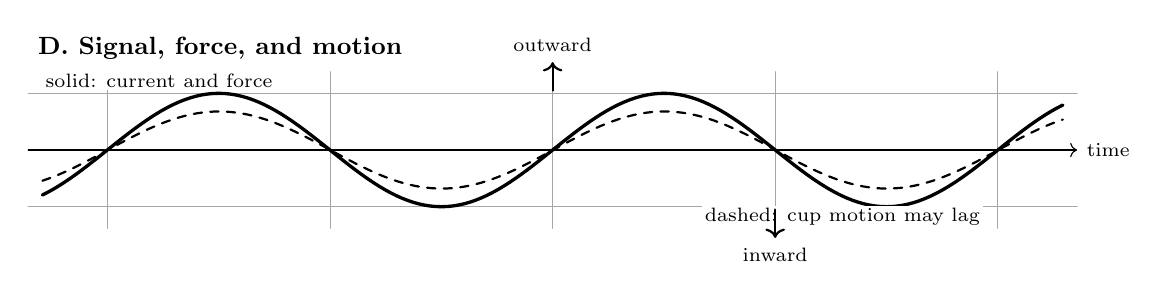
\begin{tikzpicture}[x=.90cm,y=.72cm,line cap=round,line join=round]
\node[font=\small\bfseries,anchor=west]at(-7.4,1.80){D. Signal, force, and motion};
\draw[->](-7.4,0)--(7.4,0)node[right,font=\scriptsize]{time};
\foreach \x in {-6.28,-3.14,0,3.14,6.28}
  \draw[black!35](\x,-1.38)--(\x,1.38);
\draw[black!35](-7.4,1)--(7.4,1) (-7.4,-1)--(7.4,-1);
\draw[very thick,domain=-7.2:7.2,samples=180]
  plot(\x,{sin(\x r)});
\draw[thick,dashed,domain=-7.2:7.2,samples=180]
  plot(\x,{.68*sin(\x r-.28)});
\node[font=\scriptsize,anchor=west,fill=white,inner sep=1pt]at(-7.2,1.23)
  {solid: current and force};
\node[font=\scriptsize,anchor=west,fill=white,inner sep=1pt]at(2.1,-1.18)
  {dashed: cup motion may lag};
\draw[->,thick](0,1.05)--(0,1.55)
  node[above,font=\scriptsize]{outward};
\draw[->,thick](3.14,-1.05)--(3.14,-1.55)
  node[below,font=\scriptsize]{inward};
\end{tikzpicture}
\end{center}}

\def\procedure{%
\subsection{Stage 1: prove the coil before assembly}
\begin{enumerate}
  \item With all power disconnected, scrape both wire ends bright. Measure
  resistance directly across the coil. Record \(R_{\rm coil}\). An open display
  means repair the ends; near zero means look for a bypass or meter-lead error.
  \item Gently flex each lead while watching the meter. The reading should stay
  steady. Ask: why can continuity pass while a fragile joint still fails?
\end{enumerate}

\subsection{Stage 2: assemble and inspect}
\begin{enumerate}[resume]
  \item Tape the coil concentrically to the cup base. Adult secures the magnet.
  Center the coil over the magnet without contact. Move the cup lightly by
  hand: it must travel freely, silently, and return without scraping.
  \item Adult checks that the 100 \(\Omega\) series resistor is present, the
  amplifier is battery powered and at minimum level, and bare conductors
  cannot touch. Stop for heat, odor, damaged insulation, pain, or a loose
  magnet.
\end{enumerate}

\subsection{Stage 3: first motion, then sound}
\begin{enumerate}[resume]
  \item Apply a 20--30 Hz tone briefly at minimum level. Watch a paper flag on
  the cup. Increase only until motion is visible. Does the flag reverse at the
  same rate as the signal? Do not hold the moving coil.
  \item Try 100, 250, 500, and 1000 Hz at the same source setting. Record
  whether sound is clear, faint, or distorted. If your meter reads AC volts
  reliably at that frequency, measure across the coil; otherwise mark it
  ``meter bandwidth unknown'' rather than treating the number as truth.
\end{enumerate}

\begin{center}\small
\begin{tabularx}{.94\linewidth}{@{}r r r L@{}}
\toprule
\textbf{Frequency} & \(\boldsymbol{V_{\rm coil}}\) & \textbf{Observed level} &
\textbf{Motion / quality}\\
\midrule
20--30 Hz & \rule{1.2cm}{.3pt} & \rule{1.4cm}{.3pt} & \rule{3.7cm}{.3pt}\\
100 Hz & \rule{1.2cm}{.3pt} & \rule{1.4cm}{.3pt} & \rule{3.7cm}{.3pt}\\
250 Hz & \rule{1.2cm}{.3pt} & \rule{1.4cm}{.3pt} & \rule{3.7cm}{.3pt}\\
500 Hz & \rule{1.2cm}{.3pt} & \rule{1.4cm}{.3pt} & \rule{3.7cm}{.3pt}\\
1000 Hz & \rule{1.2cm}{.3pt} & \rule{1.4cm}{.3pt} & \rule{3.7cm}{.3pt}\\
\bottomrule
\end{tabularx}
\end{center}

\subsection{Troubleshoot from evidence}
\begin{tabularx}{\linewidth}{@{}p{.25\linewidth}p{.28\linewidth}L@{}}
\toprule
\textbf{Evidence} & \textbf{Likely cause} & \textbf{Power-off check}\\
\midrule
Open resistance & Broken lead or enamel remains & Scrape ends; flex-test; find
the discontinuity.\\
Stable resistance, no motion & No signal or bad connection & Verify amplifier
on a known safe load; inspect every joint.\\
Motion but scraping & Coil off-center or magnet loose & Re-center; adult
re-secures magnet.\\
Sound only at high level & Large gap, heavy cup, weak coupling & Reduce gap
without contact; remove excess tape.\\
Buzz at one frequency & Loose tape or cup resonance & Press tape with power
off; repeat just above and below that frequency.\\
Heat, odor, distortion & Excess drive or shorted turns & Disconnect at once;
inspect and remeasure before deciding whether to retire the coil.\\
\bottomrule
\end{tabularx}

\subsection{Final proof}
Reconnect after every power-off check. A successful build must pass all four:
\begin{enumerate}[label=\(\circ\),leftmargin=1.8em]
  \item Coil resistance is finite, repeatable, and unchanged by gentle lead flex.
  \item The unpowered cup moves freely without rubbing.
  \item A low-frequency signal produces visible alternating motion.
  \item At least two commanded audio frequencies produce distinguishable,
  repeatable sound, with no heat, odor, loose magnet, or unexpected contact.
\end{enumerate}}

\def\explanation{%
The amplifier supplies changing current. In the permanent magnet's field, the
coil experiences a force whose direction follows current direction. Because
the coil is attached to the cup, the cup moves air. Steady DC can make one
displacement and heating, but not a sustained tone. Loudness need not rise with
frequency: coil impedance, cup mass and stiffness, magnetic gap, resonances,
and the ear all shape the response. The measurements separate an electrical
claim (a continuous coil receives a changing signal) from mechanical evidence
(free, alternating motion) and acoustic evidence (repeatable sound).}

\def\extension{%
Add one removable paper clip near the cup rim, then repeat only 100, 250, and
500 Hz at the unchanged source setting. Predict first. Plot two simple response
traces---frequency horizontally, observed level vertically---and circle any
frequency where the added mass changes buzz, level, or motion. A phone spectrum
display may confirm the strongest frequency, but it does not replace the
resistance, motion, and stop-line checks.

\begin{center}
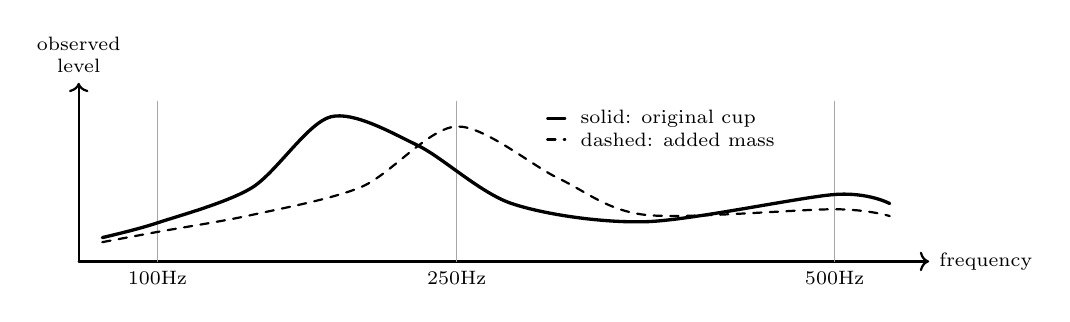
\begin{tikzpicture}[x=1cm,y=.72cm,line cap=round,line join=round]
\draw[->,thick](0,0)--(10.8,0)node[right,font=\scriptsize]{frequency};
\draw[->,thick](0,0)--(0,3.15)node[above,font=\scriptsize,align=center]
  {observed\\level};
\foreach \x/\lab in {1/100,4.8/250,9.6/500}
  {\draw[black!35](\x,0)--(\x,2.82);
   \node[font=\scriptsize,below]at(\x,0){\lab Hz};}
\draw[very thick]plot[smooth]coordinates
  {(0.3,.42)(1,.68)(2.2,1.30)(3.2,2.55)(4.3,2.05)(5.5,1.02)(7.2,.70)(9.6,1.18)(10.3,1.02)};
\draw[thick,dashed]plot[smooth]coordinates
  {(0.3,.34)(1,.52)(2.2,.82)(3.6,1.32)(4.8,2.38)(6.1,1.46)(7.2,.82)(9.6,.92)(10.3,.80)};
\node[font=\scriptsize,anchor=west]at(6.25,2.52){solid: original cup};
\node[font=\scriptsize,anchor=west]at(6.25,2.15){dashed: added mass};
\draw[thick](5.95,2.52)--(6.18,2.52);
\draw[thick,dashed](5.95,2.15)--(6.18,2.15);
\end{tikzpicture}
\end{center}

\begin{tabularx}{\linewidth}{@{}p{.16\linewidth}p{.20\linewidth}p{.20\linewidth}L@{}}
\toprule
\textbf{Frequency} & \textbf{Original level} & \textbf{With mass} &
\textbf{What changed?}\\
\midrule
100 Hz & \rule{2cm}{.3pt} & \rule{2cm}{.3pt} & \rule{3.4cm}{.3pt}\\[.6em]
250 Hz & \rule{2cm}{.3pt} & \rule{2cm}{.3pt} & \rule{3.4cm}{.3pt}\\[.6em]
500 Hz & \rule{2cm}{.3pt} & \rule{2cm}{.3pt} & \rule{3.4cm}{.3pt}\\
\bottomrule
\end{tabularx}

\smallskip
\textbf{Questions.} Did added mass move the strongest response higher or
lower? Which observation supports that claim? Was commanded frequency the same
as the strongest measured peak? Which conclusion is justified by the evidence,
and which remains only a plausible explanation?}

% Telos shared preamble.
%
% Every Telos publication is designed to be printed on a home laser printer,
% one sheet at a time, and carried into a boat or a garage. Two constraints
% follow from that and govern everything below:
%
%   1. Pure monochrome. No value is ever a hue. Emphasis is carried by rule
%      weight, fill, and type, never by color, so a grayscale or black-only
%      printer loses nothing.
%   2. Card density. A "one-pager" is a hard contract: the leaf must fit on a
%      single side of US Letter. The layout is therefore tight by default and
%      the environments below are sized to leave room for a plate.

\documentclass[10pt,letterpaper]{article}

\usepackage[margin=0.55in,includefoot,footskip=0.24in]{geometry}
\usepackage[T1]{fontenc}
\usepackage[utf8]{inputenc}
\usepackage{lmodern}
\usepackage{microtype}
\usepackage{array}
\usepackage{booktabs}
\usepackage{longtable}
\usepackage{tabularx}
\usepackage{enumitem}
\usepackage{needspace}
\usepackage{multicol}
\usepackage{ragged2e}
\usepackage{graphicx}
\usepackage{wrapfig}
\usepackage{xcolor}
\usepackage{fancyhdr}
\usepackage{titlesec}
\usepackage{hyperref}
\usepackage[most]{tcolorbox}
\usepackage{tikz}
\usetikzlibrary{arrows.meta,calc,positioning,shapes.geometric,decorations.pathmorphing,patterns,fadings}

% Semantic names are kept so a document reads intelligibly, but every value is
% black, white, or a neutral gray that survives a black-only print driver.
\definecolor{telosink}{gray}{0}
\definecolor{telospaper}{gray}{1}
\definecolor{telosrule}{gray}{0.35}
\definecolor{telosfill}{gray}{0.90}
\definecolor{telosdeep}{gray}{0.72}
\definecolor{telosmute}{gray}{0.45}

\hypersetup{hidelinks,pdfborder={0 0 0}}

% Keep an unchanged source byte-reproducible across rebuilds: no build-clock
% creation date and no random trailer ID.
\pdfinfoomitdate=1
\pdftrailerid{}

\setlength{\parindent}{0pt}
\setlength{\parskip}{0.42em}
\setlength{\tabcolsep}{4pt}
\setlength{\columnsep}{1.1em}
\renewcommand{\arraystretch}{1.18}
\setlist[itemize]{leftmargin=1.15em,itemsep=0.12em,topsep=0.2em,parsep=0pt}
\setlist[enumerate]{leftmargin=1.5em,itemsep=0.18em,topsep=0.2em,parsep=0pt}
\setlist[description]{leftmargin=0pt,itemsep=0.16em,topsep=0.2em,parsep=0pt,
  font=\normalfont\bfseries}

% ---------------------------------------------------------------------------
% Document identity. Each leaf declares these before \begin{document} so the
% running head, the colophon, and the PDF metadata all agree.
% ---------------------------------------------------------------------------
\newcommand{\TelosProject}{Telos}
\newcommand{\TelosDocTitle}{}
\newcommand{\TelosDocSubtitle}{}
\newcommand{\TelosRevision}{}

\newcommand{\telosmeta}[4]{%
  \renewcommand{\TelosProject}{#1}%
  \renewcommand{\TelosDocTitle}{#2}%
  \renewcommand{\TelosDocSubtitle}{#3}%
  \renewcommand{\TelosRevision}{#4}%
  \hypersetup{pdftitle={#2},pdfsubject={#3; version #4},
    pdfkeywords={Telos, version #4},pdfauthor={Telos}}%
}

\pagestyle{fancy}
\fancyhf{}
\renewcommand{\headrulewidth}{0pt}
\renewcommand{\footrulewidth}{0.4pt}
\fancyfoot[L]{\footnotesize\textsc{\TelosProject}}
\fancyfoot[C]{\footnotesize\TelosDocTitle}
\fancyfoot[R]{\footnotesize\thepage}

% The first page of a one-pager carries the masthead instead of a running foot,
% so its footer is the compact provenance line.
\fancypagestyle{telosfirst}{%
  \fancyhf{}%
  \renewcommand{\headrulewidth}{0pt}%
  \renewcommand{\footrulewidth}{0.4pt}%
  \fancyfoot[L]{\footnotesize\textsc{\TelosProject}}%
  \fancyfoot[C]{\footnotesize\TelosRevision}%
  \fancyfoot[R]{\footnotesize\thepage}%
}

% ---------------------------------------------------------------------------
% Masthead. A heavy rule, the title, a light subtitle, a thin rule. The
% optional argument is a right-aligned tag (a species' scientific name, a
% lesson number) that sits on the title's baseline.
% ---------------------------------------------------------------------------
\newcommand{\telosmasthead}[1][]{%
  \thispagestyle{telosfirst}%
  \begingroup
  \setlength{\parskip}{0pt}%
  \noindent\rule{\linewidth}{1.6pt}\par
  \vspace{0.30em}
  \noindent
  \begin{minipage}[b]{0.66\linewidth}
    \raggedright{\LARGE\bfseries\TelosDocTitle}
  \end{minipage}%
  \hfill
  \begin{minipage}[b]{0.32\linewidth}
    \raggedleft{\small\itshape #1}
  \end{minipage}\par
  \vspace{0.18em}
  \noindent{\small\TelosDocSubtitle}\par
  \vspace{0.28em}
  \noindent\rule{\linewidth}{0.4pt}\par
  \endgroup
  \vspace{0.35em}
}

% ---------------------------------------------------------------------------
% Headings. Compact, small-caps, rule-anchored — a card has no room for the
% article class's default vertical air.
% ---------------------------------------------------------------------------
\titleformat{\section}{\normalfont\large\bfseries}{}{0pt}{}[\vspace{-0.55em}\rule{\linewidth}{0.4pt}]
\titlespacing*{\section}{0pt}{0.85em}{0.35em}
\titleformat{\subsection}{\normalfont\normalsize\bfseries}{}{0pt}{}
\titlespacing*{\subsection}{0pt}{0.6em}{0.2em}
\titleformat{\subsubsection}{\normalfont\small\bfseries\scshape}{}{0pt}{}
\titlespacing*{\subsubsection}{0pt}{0.45em}{0.12em}

% A short run-in heading for card interiors that must not consume a full line.
\newcommand{\telosrubric}[1]{\textbf{#1}\enspace}

% Cross-reference helper. Every Telos project is a set of loose printed sheets,
% so a reference names the sheet rather than a page number.
\newcommand{\sheetref}[1]{\textit{see the \textbf{#1} sheet}}

% Which decision, ADR or sheet governs the paragraph you are reading. A reader
% who disagrees with an instruction should be able to find the reasoning behind
% it rather than having to take it on trust.
\newcommand{\governedby}[1]{{\footnotesize\textsc{governed by #1}}}

% ---------------------------------------------------------------------------
% Quantities. siunitx is not in this TeX Live split, and the guides need only a
% fixed thin space and upright units, so define that directly rather than take
% a package dependency the documented install would not satisfy.
%   \qty{9}{kV}  ->  9 kV        \unitof{kV}  ->  kV
% ---------------------------------------------------------------------------
\newcommand{\unitof}[1]{\ensuremath{\mathrm{#1}}}
\newcommand{\qty}[2]{#1\,\unitof{#2}}
\newcommand{\numrange}[2]{#1\,--\,#2}
\newcommand{\qtyrange}[3]{#1\,--\,#2\,\unitof{#3}}
% Inches and feet appear constantly in the fishing guide; keep one spelling.
\newcommand{\inch}[1]{#1\,in}
\newcommand{\feet}[1]{#1\,ft}

% ---------------------------------------------------------------------------
% Cards and boxes.
% ---------------------------------------------------------------------------

% Titled card with a hairline frame. The default card for facts a reader looks
% up rather than reads through.
\newtcolorbox{teloscard}[1]{
  enhanced, breakable,
  colback=telospaper, colframe=telosink, colbacktitle=telospaper,
  coltitle=telosink,
  boxrule=0.5pt, sharp corners,
  left=6pt, right=6pt, top=4pt, bottom=4pt,
  toptitle=3pt, bottomtitle=3pt, titlerule=0.4pt,
  before skip=6pt, after skip=6pt,
  title={#1}, fonttitle=\small\bfseries
}

% Untitled left-ruled block: hierarchy without a redundant label.
\newtcolorbox{telosframe}{
  enhanced, breakable,
  colback=telospaper, frame hidden, boxrule=0pt, sharp corners,
  borderline west={1.3pt}{0pt}{telosink},
  left=8pt, right=2pt, top=3pt, bottom=3pt,
  before skip=6pt, after skip=6pt
}

% Filled emphasis panel — the "read this first" block. The 10% fill stays
% legible under a cheap laser toner curve and still reads as distinct.
\newtcolorbox{telospanel}[1]{
  enhanced, breakable,
  colback=telosfill, colframe=telosink, colbacktitle=telosfill,
  coltitle=telosink,
  boxrule=0.5pt, sharp corners,
  left=6pt, right=6pt, top=4pt, bottom=4pt,
  toptitle=3pt, bottomtitle=3pt, titlerule=0.4pt,
  before skip=6pt, after skip=6pt,
  title={#1}, fonttitle=\small\bfseries
}

% Hazard block. Deliberately the heaviest object on any page: a 1.4pt frame
% plus a solid title bar. Nothing else in Telos is allowed to look like this,
% so a reader skimming a lesson cannot mistake it for ordinary emphasis.
\newtcolorbox{teloshazard}[1]{
  enhanced, breakable,
  colback=telospaper, colframe=telosink,
  colbacktitle=telosink, coltitle=telospaper,
  boxrule=1.4pt, sharp corners,
  left=6pt, right=6pt, top=5pt, bottom=5pt,
  toptitle=3pt, bottomtitle=3pt,
  before skip=8pt, after skip=8pt,
  title={\MakeUppercase{#1}}, fonttitle=\small\bfseries
}

% A stop-and-check gate. Used before anything destructive, and before anything
% that would be expensive to discover later. Shared by every project that has
% a procedure someone could get hurt following carelessly.
\newtcolorbox{gate}[1]{
  enhanced, breakable,
  colback=telospaper, colframe=telosink,
  boxrule=1.0pt, sharp corners,
  left=6pt, right=6pt, top=4pt, bottom=4pt,
  toptitle=3pt, bottomtitle=3pt, titlerule=0.4pt,
  before skip=7pt, after skip=7pt,
  colbacktitle=telospaper, coltitle=telosink,
  title={\MakeUppercase{#1}}, fonttitle=\small\bfseries
}

% ---------------------------------------------------------------------------
% Rating dots. A five-step scale that prints identically in black-only: filled
% versus open circles, never a shaded bar.
% ---------------------------------------------------------------------------
\newcommand{\telosdot}{\tikz[baseline=-0.42ex]\fill[telosink] (0,0) circle (0.28ex);}
\newcommand{\telosopendot}{\tikz[baseline=-0.42ex]\draw[telosink,line width=0.28pt] (0,0) circle (0.28ex);}
\makeatletter
\newcounter{telos@rate}
\newcommand{\telosrating}[1]{%
  \begingroup
  \setcounter{telos@rate}{0}%
  \@whilenum\value{telos@rate}<#1\do{\telosdot\kern0.22em\stepcounter{telos@rate}}%
  \@whilenum\value{telos@rate}<5\do{\telosopendot\kern0.22em\stepcounter{telos@rate}}%
  \endgroup
}
\makeatother

% ---------------------------------------------------------------------------
% Tables.
%
% tabularx reads its body by scanning for a literal \end{tabularx}, so it can
% never be wrapped in a \newenvironment. Documents therefore open tabularx and
% longtable directly and take their house style from these column types and the
% booktabs rules. The one exception is the fact strip below, which is built on
% plain tabular precisely so it *can* be an environment.
% ---------------------------------------------------------------------------
\newcolumntype{L}{>{\raggedright\arraybackslash}X}
\newcolumntype{R}{>{\raggedleft\arraybackslash}X}
\newcolumntype{C}{>{\centering\arraybackslash}X}
\newcolumntype{B}{>{\bfseries\raggedright\arraybackslash}X}
\newcolumntype{N}{>{\raggedright\arraybackslash}p{0.16\linewidth}}

% Key/value fact strip. Two flush columns of short lookups; the label column is
% a fixed fraction so a stack of cards aligns across the whole guide.
\newenvironment{telosfacts}[1][0.24]
  {\begingroup\small
   \setlength{\parskip}{0pt}%
   \renewcommand{\arraystretch}{1.25}%
   \begin{tabular}{@{}>{\bfseries\raggedright\arraybackslash}p{\dimexpr#1\linewidth\relax}@{\hspace{0.7em}}>{\raggedright\arraybackslash}p{\dimexpr\linewidth-#1\linewidth-0.7em\relax}@{}}}
  {\end{tabular}\par\endgroup}
\newcommand{\telosfact}[2]{#1 & #2\\}

% ---------------------------------------------------------------------------
% Seasonal / diurnal activity bar.
%
% \telosseasonbar{4,3,2,1,1,2,3,3,4,5,4,3} draws a twelve-cell month strip
% where each value 0-5 is a fill height. Height, not gray value, carries the
% signal, so it is exact under any toner curve; the cell is outlined either way
% so an empty month is still visibly a month.
% ---------------------------------------------------------------------------
\newcommand{\telosseasonlabels}{J,F,M,A,M,J,J,A,S,O,N,D}
\newcommand{\telosseasonbar}[1]{%
  \begingroup
  \begin{tikzpicture}[x=1.25em,y=2.1ex,baseline=0pt]
    \foreach \v [count=\i from 0] in {#1} {
      \draw[telosrule,line width=0.3pt] (\i,0) rectangle (\i+0.86,5);
      \ifnum\v>0
        \fill[telosink] (\i,0) rectangle (\i+0.86,\v);
      \fi
    }
    \foreach \m [count=\i from 0] in \telosseasonlabels {
      \node[font=\tiny,anchor=north,inner sep=1.2pt] at (\i+0.43,-0.1) {\m};
    }
  \end{tikzpicture}%
  \endgroup
}

% Four-cell day-part strip: dawn, midday, dusk, night.
\newcommand{\telosdaylabels}{Dawn,Mid,Dusk,Night}
\newcommand{\telosdaybar}[1]{%
  \begingroup
  \begin{tikzpicture}[x=2.9em,y=2.1ex,baseline=0pt]
    \foreach \v [count=\i from 0] in {#1} {
      \draw[telosrule,line width=0.3pt] (\i,0) rectangle (\i+0.92,5);
      \ifnum\v>0
        \fill[telosink] (\i,0) rectangle (\i+0.92,\v);
      \fi
    }
    \foreach \m [count=\i from 0] in \telosdaylabels {
      \node[font=\tiny,anchor=north,inner sep=1.2pt] at (\i+0.46,-0.1) {\m};
    }
  \end{tikzpicture}%
  \endgroup
}

% A bar needs vertical room for its labels when it sits in a fact strip.
\newcommand{\telosbarrow}[1]{\rule{0pt}{4.2ex}#1\rule[-1.6ex]{0pt}{1.6ex}}

% ---------------------------------------------------------------------------
% Plates. A species or apparatus illustration with a caption rule beneath it.
% \telosplate{width fraction}{file}{caption}
% ---------------------------------------------------------------------------
\newcommand{\telosplate}[3]{%
  \begingroup
  \centering
  \includegraphics[width=#1\linewidth]{#2}\par
  \vspace{0.15em}
  \begin{minipage}{#1\linewidth}
    \rule{\linewidth}{0.4pt}\par
    \vspace{0.1em}
    {\footnotesize #3\par}
  \end{minipage}\par
  \endgroup
  \vspace{0.3em}
}

% TikZ drawing conventions shared by every rig, knot, and circuit diagram.
\tikzset{
  telos line/.style={draw=telosink,line width=0.7pt},
  telos hair/.style={draw=telosink,line width=0.35pt},
  telos heavy/.style={draw=telosink,line width=1.2pt},
  telos node/.style={draw=telosink,fill=telospaper,align=center,inner sep=4pt,font=\small},
  telos emphasis/.style={draw=telosink,line width=1.2pt,fill=telospaper,align=center,
    inner sep=4pt,font=\small\bfseries},
  telos label/.style={font=\scriptsize,inner sep=1.5pt},
  telos arrow/.style={-{Stealth[length=1.8mm]},draw=telosink,line width=0.6pt},
  telos dim/.style={|<->|,draw=telosink,line width=0.35pt},
  telos water/.style={draw=telosrule,line width=0.4pt,decorate,
    decoration={snake,amplitude=0.4mm,segment length=3mm}},
}

% ---------------------------------------------------------------------------
% Lesson furniture
% ---------------------------------------------------------------------------

% \lessonhead{number}{time}{who does what}
\newcommand{\lessonhead}[3]{%
  \par\noindent
  \begin{minipage}{\linewidth}
    \rule{\linewidth}{0.4pt}\par
    \vspace{0.3em}
    {\small\textbf{Lesson #1}\quad$\cdot$\quad #2\quad$\cdot$\quad #3\par}
    \vspace{0.25em}
    \rule{\linewidth}{0.4pt}
  \end{minipage}\par
  \vspace{0.5em}}

% The materials list. Two columns of short lines; a lesson that needs a long
% shopping list is a lesson that has not been thought through.
\newenvironment{materials}
  {\begin{telospanel}{What you need}\begin{multicols}{2}
   \begin{itemize}[leftmargin=1em,itemsep=0.05em,topsep=0pt]}
  {\end{itemize}\end{multicols}\end{telospanel}}

% The four rubrics every lesson carries, in the same order every time:
% what you are about to see, what to do, what it means, and what to ask.
\newcommand{\lessonsection}[1]{\section*{#1}\vspace{-0.35em}\rule{\linewidth}{0.4pt}\vspace{0.2em}}

% A prediction box. The point of the curriculum is that they commit to an
% answer before the demonstration, not after.
\newtcolorbox{predict}{
  enhanced, breakable,
  colback=telospaper, colframe=telosink,
  boxrule=0.5pt, sharp corners,
  left=6pt, right=6pt, top=4pt, bottom=4pt,
  before skip=6pt, after skip=6pt,
  borderline west={2.2pt}{0pt}{telosink},
  title={\small\bfseries Predict first}, fonttitle=\small\bfseries,
  colbacktitle=telospaper, coltitle=telosink,
  toptitle=3pt, bottomtitle=3pt, titlerule=0.4pt,
}

% ---------------------------------------------------------------------------
% Colophon. Rendered once, at the end of the last page, in the recovered footer
% area so it never creates a page of its own.
% ---------------------------------------------------------------------------
\newif\ifTelosColophonRendered
\newcommand{\TelosColophonExtra}{}
\newcommand{\TelosColophon}{%
  \ifTelosColophonRendered\else
  \global\TelosColophonRenderedtrue
  \par
  \enlargethispage{0.5in}%
  \vspace{0.3em}%
  \begingroup
  \setlength{\parskip}{0pt}%
  \begin{minipage}{\linewidth}
  \rule{\linewidth}{0.35pt}\par
  \vspace{0.3em}%
  \fontsize{7}{8.2}\selectfont
  \textbf{Telos.} \TelosProject{} — \TelosDocTitle. Revised \TelosRevision.
  \TelosColophonExtra{}
  Project-created text and diagrams are licensed \href{https://creativecommons.org/licenses/by/4.0/}{CC BY 4.0}.
  Incorporated public-domain artwork remains public domain and is credited on
  the plate it appears with. See \texttt{LICENSE} and \texttt{CREDITS.md} in the
  source. Nothing here is professional advice; verify current regulations and
  follow the stated safety procedure.
  \end{minipage}
  \endgroup
  \fi
}
\AtEndDocument{\TelosColophon}

\newcommand{\editiontag}{ChatGPT edition}
\newcommand{\boundary}{\textbf{Learner boundary:} isolated battery power only,
12 V DC maximum. No outlets, mains leads, opened appliances, large battery
packs, charged power capacitors, ignition coils, sparks, or exposed high
voltage. An adult facilitator is not thereby an electrically qualified person.}
\newenvironment{recordbox}{\begin{teloscard}{Evidence record}\small
\begin{tabularx}{\linewidth}{@{}p{.19\linewidth}L@{}}
Prediction & \rule{.95\linewidth}{.3pt}\\[1.1em]
One change & \rule{.95\linewidth}{.3pt}\\[1.1em]
Observation & \rule{.95\linewidth}{.3pt}\\[1.1em]
Claim + because & \rule{.95\linewidth}{.3pt}
\end{tabularx}}{\end{teloscard}}
\newcommand{\sourcefoot}{\par\smallskip{\footnotesize Physics and safety basis:
NIST SI/CODATA; OSHA 29 CFR 1910.333 and OSHA 3075; DOE Electrical Science
handbooks; HyperPhysics (Georgia State University); University of Colorado
PhET teacher resources. Full citations and scope notes are recorded in the
provider-neutral electricity research library.}}
\newcommand{\rolecard}{\begin{telospanel}{Stop line and roles}\boundary\par
\smallskip The learner predicts, assembles only the pictured battery circuit,
and records. The adult inspects parts, controls power, and stops heat, odor,
damage, pain, or unexpected behavior. Work outside this boundary belongs only
to a person qualified for that work.\end{telospanel}}
\newcommand{\circuitdiagram}{\begin{center}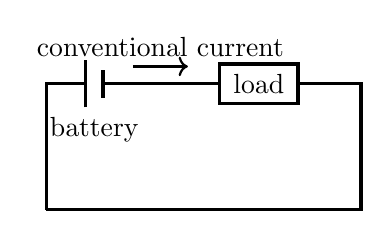
\begin{tikzpicture}[x=1cm,y=1cm]
\draw[very thick] (0,0)--(0,1.6)--(.5,1.6);
\draw[very thick] (.5,1.3)--(.5,1.9); \draw[very thick] (.72,1.42)--(.72,1.78);
\node[below] at (.61,1.3){battery};
\draw[very thick] (.72,1.6)--(2.2,1.6);
\draw[very thick] (2.2,1.35) rectangle (3.2,1.85);
\node at (2.7,1.6){load};
\draw[very thick] (3.2,1.6)--(4,1.6)--(4,0)--(0,0);
\draw[->,thick] (1.1,1.82)--(1.8,1.82) node[midway,above]{conventional current};
\end{tikzpicture}\end{center}}
\newcommand{\fielddiagram}{\begin{center}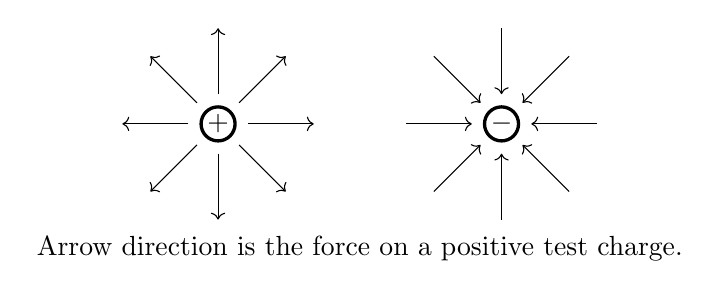
\begin{tikzpicture}[scale=.9]
\draw[very thick] (0,0) circle (.24); \node at (0,0){$+$};
\foreach \a in {0,45,...,315}{\draw[->] ({.42*cos(\a)},{.42*sin(\a)})--({1.35*cos(\a)},{1.35*sin(\a)});}
\draw[very thick] (4,0) circle (.24); \node at (4,0){$-$};
\foreach \a in {0,45,...,315}{\draw[<-] ({4+.42*cos(\a)},{.42*sin(\a)})--({4+1.35*cos(\a)},{1.35*sin(\a)});}
\node[below] at (2,-1.45){Arrow direction is the force on a positive test charge.};
\end{tikzpicture}\end{center}}
\newcommand{\coildiagram}{\begin{center}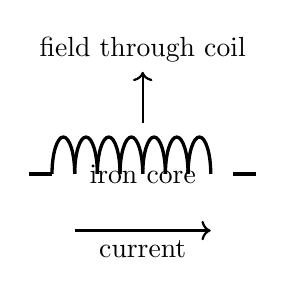
\begin{tikzpicture}[x=.72cm,y=.72cm]
\draw[very thick] (-2,0)--(-1.6,0);
\foreach \x in {-1.6,-1.2,...,1.2}{\draw[very thick] (\x,0) arc (180:0:.2 and .65);}
\draw[very thick] (1.6,0)--(2,0);
\draw[->,thick] (-1.2,-1)--(1.2,-1) node[midway,below]{current};
\draw[->,thick] (0,.9)--(0,1.8) node[above]{field through coil};
\node at (0,0){iron core};
\end{tikzpicture}\end{center}}
\newcommand{\inductiondiagram}{\begin{center}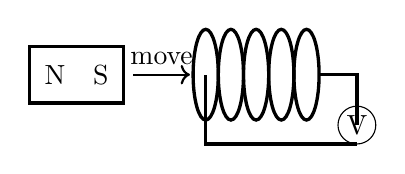
\begin{tikzpicture}[x=.8cm,y=.8cm]
\draw[very thick] (-2,-.45) rectangle (-.5,.45); \node at (-1.25,0){N\quad S};
\draw[->,thick] (-.35,0)--(.55,0) node[midway,above]{move};
\foreach \x in {.8,1.2,...,2.4}{\draw[very thick] (\x,0) ellipse (.2 and .72);}
\draw[very thick] (2.6,0)--(3.2,0)--(3.2,-.8);
\draw (3.2,-.8) circle (.3); \node at (3.2,-.8){V};
\draw[very thick] (3.2,-1.1)--(.8,-1.1)--(.8,0);
\end{tikzpicture}\end{center}}

\telosmeta{Electricity \& Magnetism}{\doctitle}{\docsubtitle}{20260726.001}
\begin{document}
\telosmasthead[\editiontag\ --- \docstrap]
\rolecard
\begin{materials}\materialslist\end{materials}
\begin{predict}\prediction\end{predict}
\diagram
\section{Investigate}
\procedure
\section{Explain from the evidence}
\explanation
\section{Change one thing}
\extension
\begin{recordbox}\end{recordbox}
\sourcefoot
\end{document}

